\documentclass[usenames,dvipsnames,15pt]{beamer}

\newcommand{\backupbegin}{
   \newcounter{finalframe}
   \setcounter{finalframe}{\value{framenumber}}
}
\newcommand{\backupend}{
   \setcounter{framenumber}{\value{finalframe}}
}

\usepackage{natbib}
\bibliographystyle{natbib}

\usepackage{xcolor,cancel}
\newcommand\hcancel[2][black]{\setbox0=\hbox{$#2$}%
\rlap{\raisebox{.45\ht0}{\textcolor{#1}{\rule{\wd0}{1pt}}}}#2} 


\usepackage{hyperref}
\usepackage{setspace}
\usepackage{tikz}
\usepackage[percent]{overpic}
\usetikzlibrary{calc,trees,positioning,arrows,fit,shapes,calc}
\usepackage{verbatim}
\usepackage{stmaryrd}
\usepackage{amsmath}
\usepackage{amssymb}
\usepackage{colortbl}
\usepackage{nicefrac}

\usepackage{color}
\usepackage[percent]{overpic}
\usepackage{kbordermatrix}


\definecolor{fgreen}{RGB}{34,139,34}

\newcommand{\N}{G}
\newcommand{\n}{g}
\newcommand{\cK}{{\color{RoyalBlue}K}}
\newcommand{\cN}{{\color{BrickRed}G}}
\newcommand{\cn}{{\color{BrickRed}g}}
\newcommand{\cS}{{\boldsymbol{S}}}

\newcommand{\cbo}{\color{BurntOrange}}
\newcommand{\crb}{\color{RoyalBlue}}
\newcommand{\cbr}{\color{BrickRed}}
\newcommand{\logistic}{\text{logistic}}

\newcommand{\yan}{\text{\Large $R$\hspace*{-.05cm}}_{{\crb A}{\cbr \n}}}
\newcommand{\ybn}{\text{\Large $R$\hspace*{-.05cm}}_{{\crb B}{\cbr \n}}}
\newcommand{\ycn}{\text{\Large $M$\hspace*{-.05cm}}_{{\cbr g}}}

\newcommand{\yana}{\text{\Large $R$\hspace*{-.05cm}}_{{\crb A}\na}}
\newcommand{\ybna}{\text{\Large $R$\hspace*{-.05cm}}_{{\crb B}\na}}
\newcommand{\ycna}{\text{\Large $M$\hspace*{-.05cm}}_{\na}}

\newcommand{\yanb}{\text{\Large $R$\hspace*{-.05cm}}_{{\crb A}\nb}}
\newcommand{\ybnb}{\text{\Large $R$\hspace*{-.05cm}}_{{\crb B}\nb}}
\newcommand{\ycnb}{\text{\Large $M$\hspace*{-.05cm}}_{\nb}}


\newcommand{\ean}{\text{\Large $\widetilde{R}$}_{{\crb A}{\cbr g}}}
\newcommand{\ebn}{\text{\Large $\widetilde{R}$}_{{\crb B}{\cbr g}}}
\newcommand{\ecn}{\text{\Large $\widetilde{M}$}_{{\cbr g}}}

\newcommand{\eana}{\text{\Large $\widetilde{R}$}_{{\crb A}{\cbr a}}}
\newcommand{\ebna}{\text{\Large $\widetilde{R}$}_{{\crb B}{\cbr a}}}
\newcommand{\ecna}{\text{\Large $\widetilde{M}$}_{{\cbr a}}}
\newcommand{\eanb}{\text{\Large $\widetilde{R}$}_{{\crb A}{\cbr b}}}
\newcommand{\ebnb}{\text{\Large $\widetilde{R}$}_{{\crb B}{\cbr b}}}
\newcommand{\ecnb}{\text{\Large $\widetilde{M}$}_{{\cbr b}}}


\newcommand{\epsan}{\text{\Large $\epsilon$}_{{\crb A}{\cbr g}}}
\newcommand{\epsbn}{\text{\Large $\epsilon$}_{{\crb B}{\cbr g}}}
\newcommand{\epscn}{\text{\Large $\epsilon$}_{{\cbr g}}}

\newcommand{\epsana}{\text{\Large $\epsilon$}_{{\crb A}{\cbr a}}}
\newcommand{\epsbna}{\text{\Large $\epsilon$}_{{\crb B}{\cbr a}}}
\newcommand{\epscna}{\text{\Large $\epsilon$}_{{\cbr a}}}
\newcommand{\epsanb}{\text{\Large $\epsilon$}_{{\crb A}{\cbr b}}}
\newcommand{\epsbnb}{\text{\Large $\epsilon$}_{{\crb B}{\cbr b}}}
\newcommand{\epscnb}{\text{\Large $\epsilon$}_{{\cbr b}}}


\newcommand{\xa}{\xi_{\crb A}}
\newcommand{\xb}{\xi_{\crb B}}

\newcommand{\na}{{\cbr a}}
\newcommand{\nb}{{\cbr b}}
\newcommand{\tn}{\text{\Large $\theta$}_{\cbr g}}
\newcommand{\tna}{\text{\Large $\theta$}_{\cbr a}}
\newcommand{\tnb}{\text{\Large $\theta$}_{\cbr b}}

\newcommand{\yca}{\text{\Large $M$\hspace*{-.05cm}}_{\na}}
\newcommand{\ycb}{\text{\Large $M$\hspace*{-.05cm}}_{\nb}}
\newcommand{\yaa}{\text{\Large $R$\hspace*{-.05cm}}_{{\crb A}\na}}
\newcommand{\ybb}{\text{\Large $R$\hspace*{-.05cm}}_{{\crb B}\nb}}

\newcommand{\pa}{\text{\Large $p$}_{\crb A}}
\newcommand{\pb}{\text{\Large $p$}_{\crb B}}

\newcommand{\slope}{\text{\Large $\gamma$}}
\newcommand{\slopehat}{\text{\Large $\widehat{\slope}$}}

\newcommand{\phat}[1]{\widehat{p_{\crb #1}}}
\newcommand{\pbar}[1]{\overline{p_{\crb #1}}}
\newcommand{\ybar}[1]{\overline{Y_{\cbr G_{#1}}}}
\newcommand{\zbar}[1]{\overline{Z_{\cbr G_{#1}}}}
\newcommand{\ebar}[1]{\overline{\epsilon_{\G_{#1}}}}
\newcommand{\ptilde}[1]{\widetilde{p_{#1}}}
\newcommand{\sm}[1]{\sigma_2^{#1}}

\newcommand{\ponehat}{\phat{1}}
\newcommand{\ptwohat}{\phat{2}}
\newcommand{\pkhat}{\phat{k}}
\newcommand{\pkt}{\ptilde{k}}
\newcommand{\pkb}{\pbar{k}}
\newcommand{\ptb}{\pbar{t}}
\newcommand{\ptt}{\ptilde{t}}
\newcommand{\ykbar}{\ybar{k}}
\newcommand{\zkbar}{\zbar{k}}
\newcommand{\ekbar}{\ebar{k}}
\newcommand{\smk}{\sm{k}}

\newcommand{\pthat}{\phat{t}}
\newcommand{\ytbar}{\ybar{t}}
\newcommand{\ztbar}{\zbar{t}}
\newcommand{\etbar}{\ebar{t}}
\newcommand{\smt}{\sm{t}}



\usetheme[numbering=fraction,progressbar=frametitle,background=light,sectionpage=progressbar]{metropolis}
\title{Estimating Cell-type Proportions Using Gene Expressions}
\author{Greg Hunt${}^1$, Saskia Freytag${}^{2,3}$, Melanie Bahlo${}^{2,3}$ and Johann Gagnon-Bartsch${}^1$}
\institute{${}^1$Statistics at the University of Michigan\\
  ${}^2$Population Health and Immunity Division at the Walter and Eliza Hall Institute of Medical Research\\ 
  ${}^3$Department of Medical Biology at the University of Melbourne}
\date{\today}

\usepackage{remreset}% tiny package containing just the \@removefromreset command
\makeatletter
\@removefromreset{subsection}{section}
\makeatother
\setcounter{subsection}{0}

\setbeamercolor{background canvas}{bg=white}

\begin{document}


{\setbeamertemplate{footline}{} 
\begin{frame}[noframenumbering]
\titlepage
\end{frame}

\begin{frame}[noframenumbering]
  \frametitle{Estimating Cell-type Proportions Using Gene Expressions}
  \hspace{1.6cm}Saskia\hspace*{2.9cm}Melanie\hspace{1.5cm} Johann\\\hspace{1.5cm}Freytag${}^{2,3}$\hspace{2.5cm}Bahlo${}^{2,3}$\hspace{.75cm} Gagnon-Bartsch${}^{1}$\\\vspace{.1cm}
  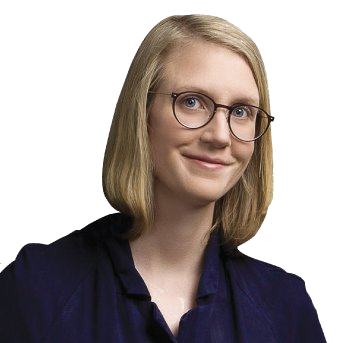
\includegraphics[scale=.33]{pictures/saskia.jpg}
  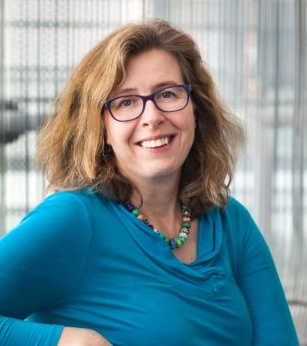
\includegraphics[scale=.33]{pictures/melanie.jpg}
  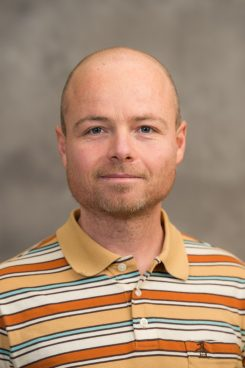
\includegraphics[scale=.31]{pictures/johann.jpg}

  \vspace{.25cm}
  {\scriptsize ${}^1$Statistics at the University of Michigan\\
  ${}^2$Population Health and Immunity Division at the Walter and Eliza Hall Institute of Medical Research\\
  ${}^3$Department of Medical Biology at the University of Melbourne}
\end{frame}

\begin{frame}[noframenumbering]
  \section{Genomics In One Slide}
  \begin{center}
    i.e. ``what is gene expression data?''
  \end{center}
\end{frame}
}

\begin{frame}
  \frametitle{Gene = Code Telling Cell How to Do Something}
             \uncover<2->{{\Large Gene is expressed = Gene used by cell}\\}
             \uncover<3->{{\Large Gene expressions $\approx$ what cells are doing}}\\
             \uncover<4->{{\Large \alert{Measure gene exprs. to learn what cells are doing.}}}

             
  \uncover<5->{{\large {\bf How?} Gene Expressed $\rightarrow$ \alert{mRNA transcript} created}\\}
  \uncover<6->{\begin{center}
    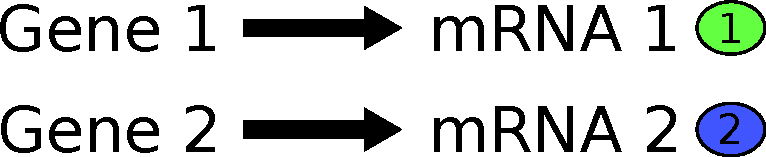
\includegraphics[scale=.35]{pictures/mrna}
  \end{center}}
  \uncover<7->{{\bf Measuring Gene Expression = Quantifying mRNA transcripts}\\}
  \uncover<8->{\begin{center}
    \vspace{-.9cm}\hspace*{-.75cm}\includegraphics[scale=.26]{pictures/measure_expr}
  \end{center}}


\end{frame}


\section{Estimating Cell-type Proportions}

\begin{frame}
  \frametitle{``De-Mixing'' = Estimating Cell-type Proportions}
  \alert{\large Given:} Gene Expression Profiles (GEPs) of:
  \begin{enumerate}
  \item sample that is mixture of cell types A,B,C,...Z
  \item reference samples of types A,B,C,...,Z\\
  \end{enumerate}
  \hspace{1cm}\begin{center}
    \begin{overprint}
      \onslide<1|handout:0>\hspace{-.75cm}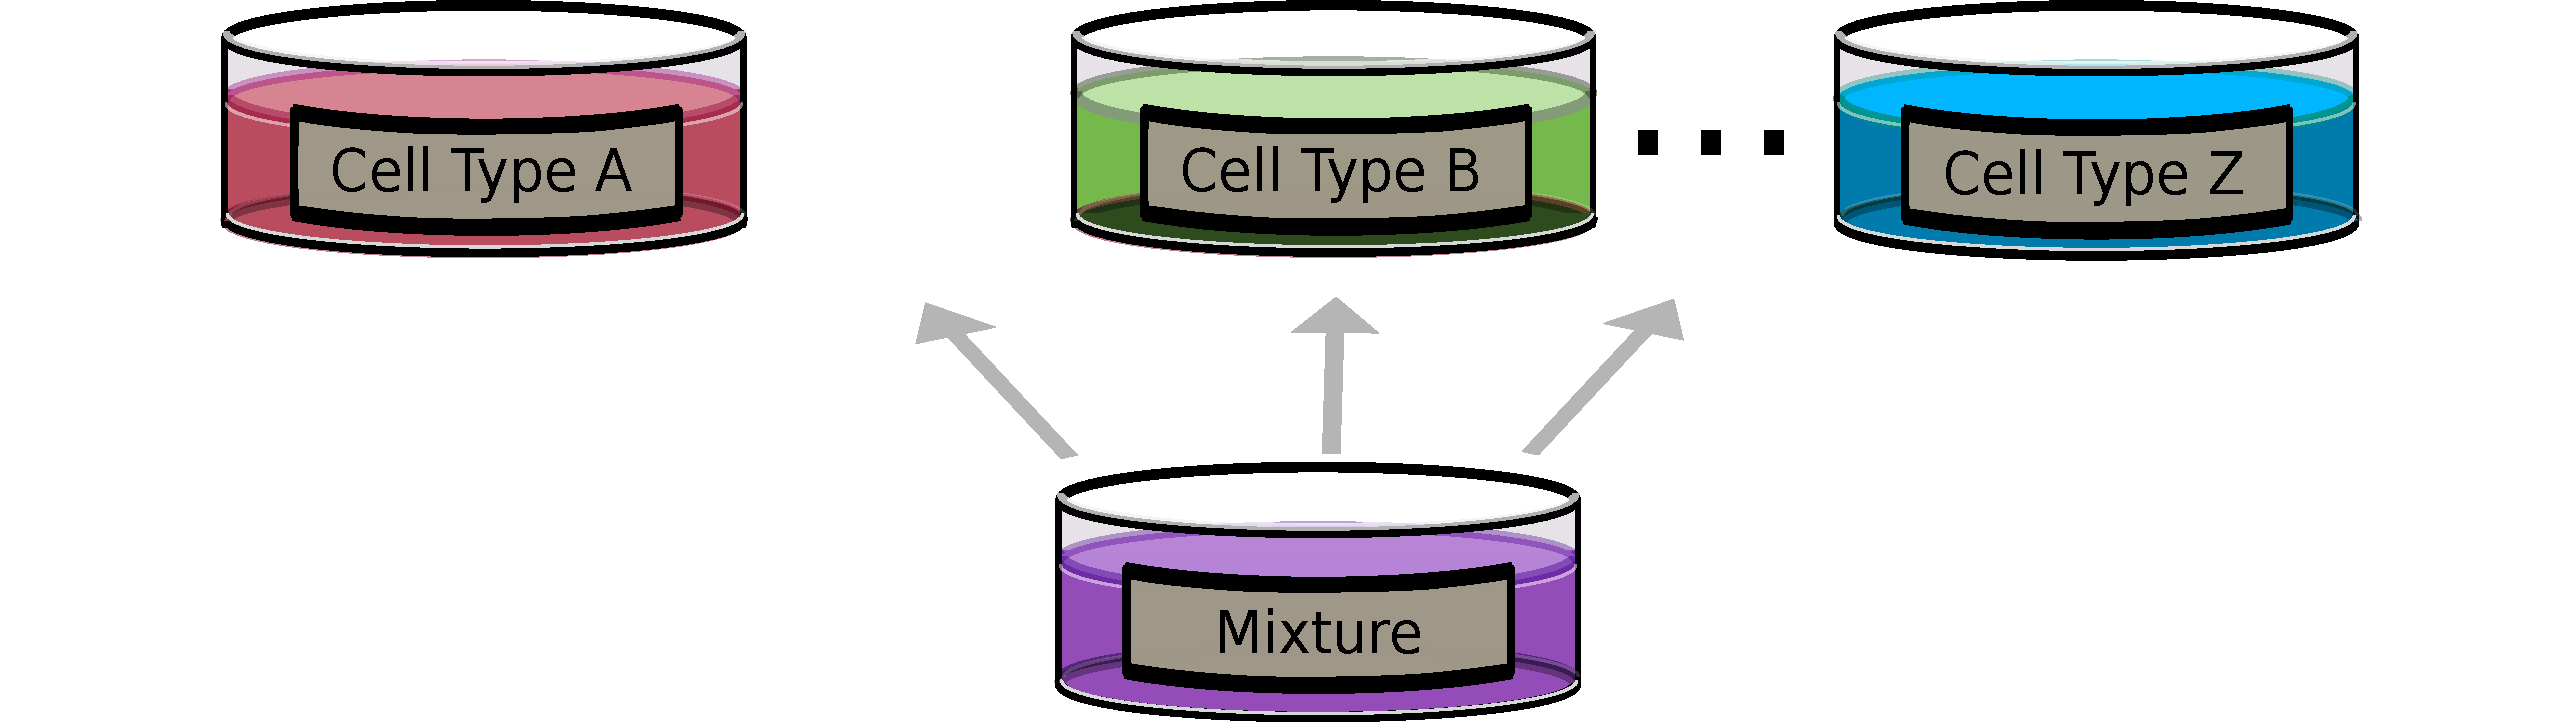
\includegraphics[scale=.28]{pictures/mixture_cartoon}
      \onslide<2-|handout:0>\hspace*{-.77cm}\includegraphics[scale=.28]{pictures/mixture_cartoon_data}
    \end{overprint}
  \end{center}
  \alert{\large Goal:} Computationally ``De-Mix'' = estimate cell-type proportions
  {\scriptsize \begin{center}\begin{tabular}{c||c|c|c|c|c}
      & \bf Type A& \bf Type B& $\cdots$& \bf Type Y&\bf  Type Z\\\hline\hline
    \bf Mixture& 5\%& 20\%& $\cdots$& 30\%& 0\%
  \end{tabular}\end{center}}
\end{frame}

\begin{frame}
  \frametitle{Why Are Cell-type Proportions Important?}
    {\Large\alert{ Broad goal:}\\\begin{center} Understand biological mechanisms of disease\\ using \alert{genetics} (or epigenetics, proteomics, ...) .\end{center}}
    {\Large\alert{ Specific goal:}}
    \begin{enumerate}
    \item Understanding changes in cell type proportions over the course of a disease
    \item Adjusting gene expression comparison between samples
    \end{enumerate}
\end{frame}

\begin{frame}
  \frametitle{Understanding Chronic Lyme}
  \begin{columns}
    \begin{column}{.25\textwidth}
      \begin{figure}
        \vspace{-.5cm}
        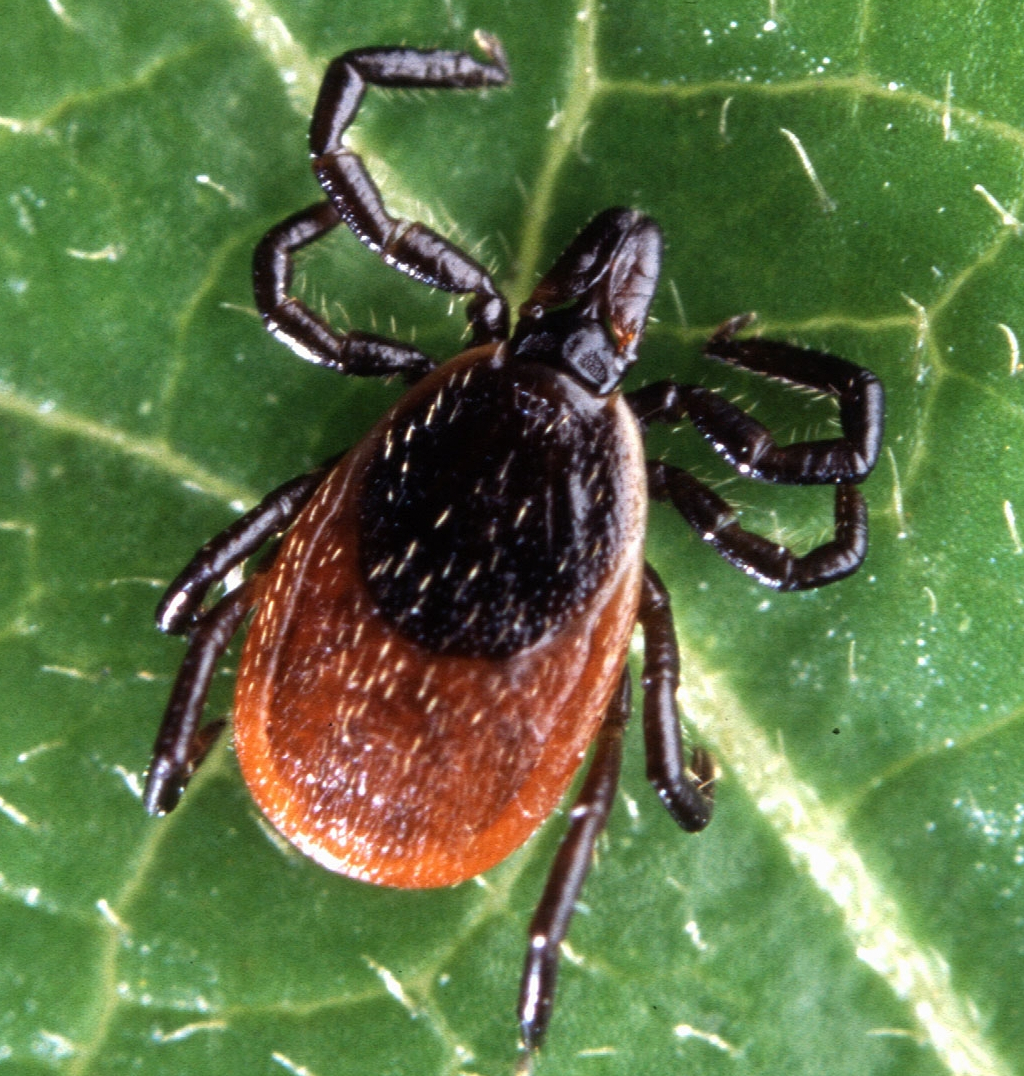
\includegraphics[scale=.35]{pictures/tick.jpg}\\
        {\tiny Adult deer tick.\\\vspace{-.2cm}\emph{Scott Bauer} [1].}
      \end{figure}\vspace{-1.25cm}
      \begin{figure}
        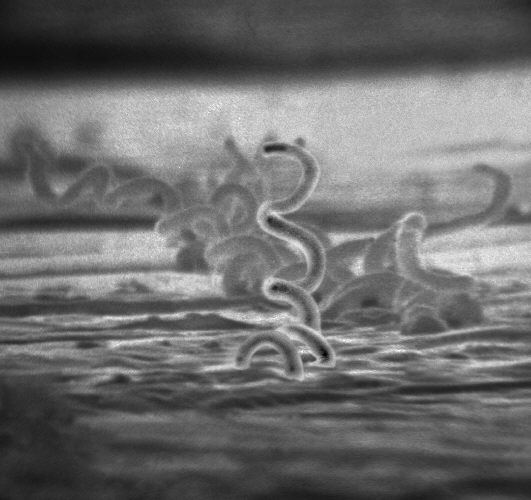
\includegraphics[scale=1.4]{pictures/spiro.jpg}\\
        {\tiny A typical spirochete.\\\vspace{-.2cm}\emph{CDC/Dr. David Cox} [2].}
      \end{figure}
    \end{column}
    \begin{column}{.75\textwidth}
      \vspace{0cm}

      {\bf Lyme disease:} bacterial infection spread by ticks.
      \begin{enumerate}
      \item {\bf acute stage} treatable with antibiotics
      \item {\bf chronic problems not well understood:} \alert{even after treatment} some patients report fatigue, arthritis, muscle soreness
      \end{enumerate}
      
      \uncover<2->{\vspace{.5cm}{\bf hypothesis:} Chronic Lyme is our own white blood cells (WBCs) attacking our own body (auto-immunity) \\\vspace{.5cm}
          
      \begin{center}\alert{{\bf c.f. Bouquet et al.}}\end{center}}
    \end{column}
  \end{columns}
\end{frame}

\begin{frame}
  \frametitle{WBCs $\rightarrow$ Immune Response $\overset{?}{\rightarrow}$ Chronic Lyme}
             {\bf Bouquet et al:} investigate theory by collecting GEPs of WBCs of 
             \begin{enumerate}
             \item \alert{28 Lyme patients} (15 resolved, 13 chronic)
             \item and \alert{13 healthy controls}.
             \end{enumerate}

             The analysis compares GEPs of all WBCs across groups.\\

             \vspace{.5cm}\uncover<2->{\alert{WBCs encompass many types:} B,T,NK,monocytes,...\\
               {\bf Understanding these sub-types is important:}

               \begin{enumerate}
               \item tracking subtype composition changes over disease course
               \item de-confounding GEP comparisons across groups (DEA)
               \end{enumerate}

             }
\end{frame}

\begin{frame}
  \frametitle{Cell-types Can Confound Differential Expression Analysis}
  \begin{columns}
    \begin{column}{.6\textwidth}
  \begin{center}\begin{minipage}{\columnwidth}
    \centering
    \begin{overprint}
      \onslide<1|handout:0>\includegraphics[scale=.38]{pictures/confound}
      \onslide<2-|handout:0>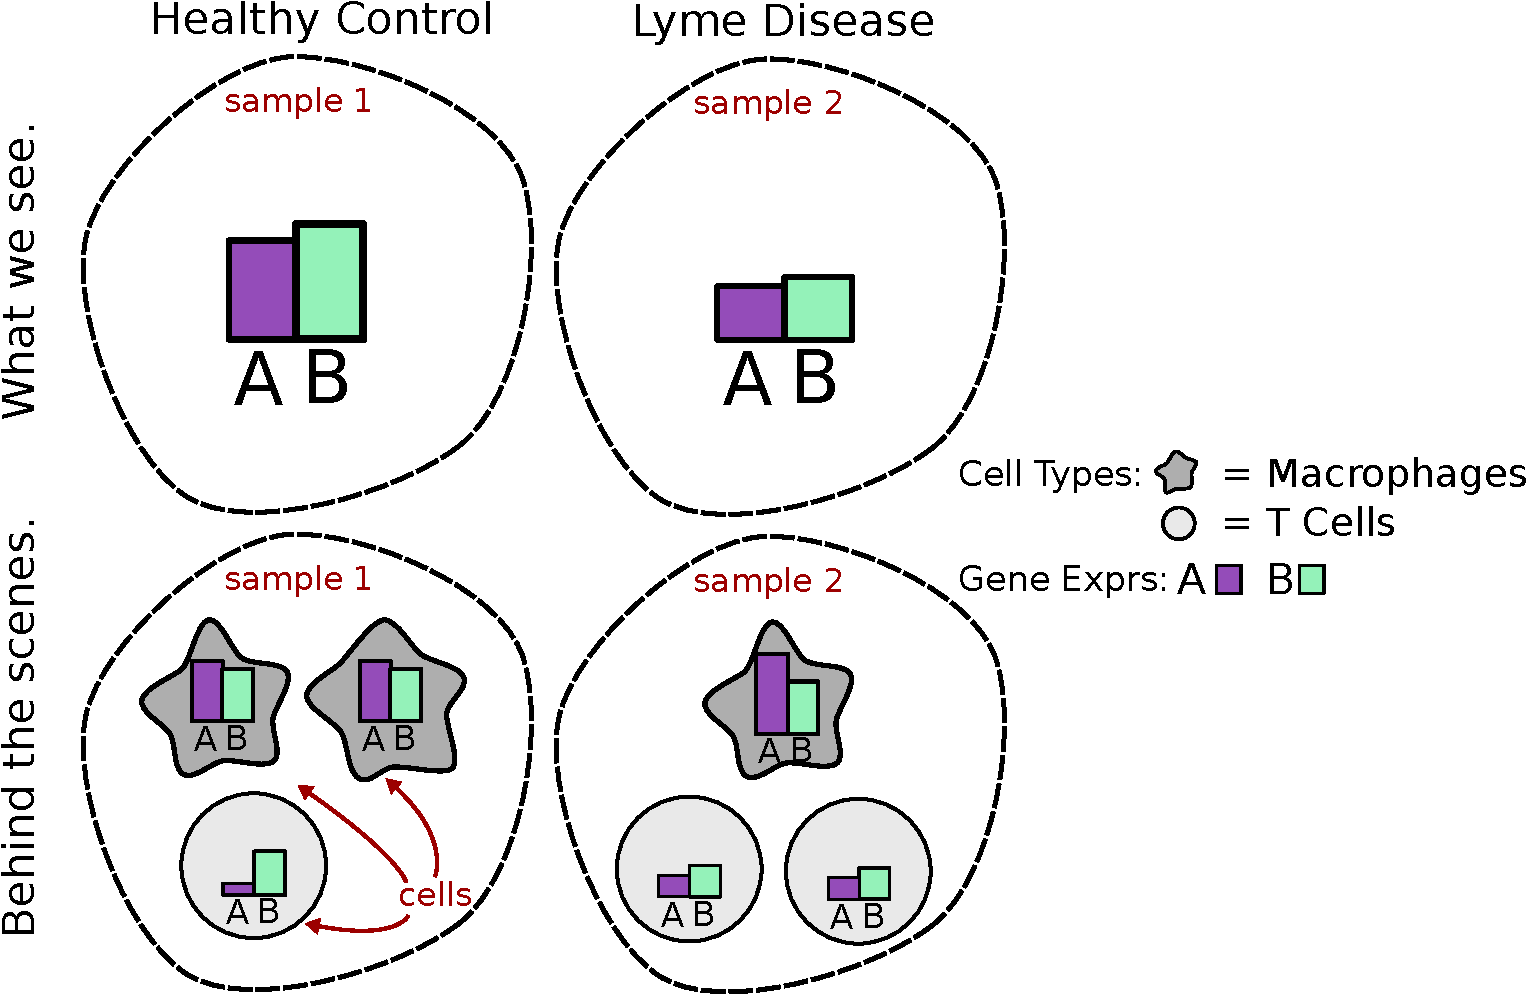
\includegraphics[scale=.38]{pictures/confound2}
    \end{overprint}
  \end{minipage}
  \end{center}
    \end{column}
    \begin{column}{.4\textwidth}\vspace{-1.7cm}

      \uncover<5->{\alert{\bf Solution:} Estimate the cell-type proportions.\\De-confound analysis with estimates.}\vspace{1.8cm}
      
    \end{column}
  \end{columns}
  \uncover<3->{Differences we see come from \vspace{-.35cm}}
  \begin{enumerate}
  \uncover<3->{\item \alert{differences across samples of GEPs for each cell type}}
  \uncover<4->{\item \alert{differences across samples of cell-type composition}}
  \end{enumerate}\vspace{-.3cm}
\end{frame}

\setcounter{subsection}{0}
\section{Previous Work}
\subsection{}

\begin{frame}
  \frametitle{A Linear Model is Commonly Used}
  General model: $M \approx PR$,  predict $P$ with known $M$ and $R$
  %$\overbrace{\text{mixture expressions}}^{M} \approx \overbrace{\text{mixture proportions}}^{P} \,\overbrace{\text{reference expressions}}^{R}$
  %(m)ixture expression $\approx$ mixture (p)roportions\, (r)eference expressions
  \vspace{-.25cm}
  \renewcommand{\arraystretch}{0.6}
  \setlength\arraycolsep{1pt}
  \renewcommand{\kbldelim}{[}% Left delimiter
  \renewcommand{\kbrdelim}{]}% Right delimiter
  \small\vspace{-.5cm}

  \[\begin{aligned}
  \hspace{-.8cm}\overset{\text{\Large M}}{\underbrace{\kbordermatrix{
    & \cbr gene_1 & \cbr gene_2 & \cbr \cdots & \cbr gene_\N \\
    \bf sample_1&  \cbo6.6 & 8.9 & \cdots & 3.5 \\
    \bf sample_2& 3.2 & 5.4 & \cdots & 4.8 \\
    \bf sample_3&  7.3& 7.7& &  &  \\
    \bf \vdots& \vdots&   & \ddots &  \\
    \bf sample_S& 4.1  &  &  &
  }}_{\text{\large mixture expressions}}}\hspace{-.1cm}\approx\hspace{-.05cm}
   &\overset{\text{\Large P}}{\underbrace{\kbordermatrix{
    & \crb type_1 & \crb type_2 & \crb\cdots & \crb type_K \\
    \bf sample_1&  \cbo.5 & \cbo.2 & \cbo\cdots & \cbo.1 \\
    \bf sample_2& 0 & .01 & \cdots & .95 \\
    \bf sample_3&  .35& .45& &  0\\
    \bf \vdots& \vdots&   & \ddots &  \\
    \bf sample_S& .1  &  &  & 
  }}_{\text{\large mixing proportions}}}
  \overset{\text{\Large R}}{\underbrace{\kbordermatrix{
    & \cbr gene_1 & \cbr gene_2 & \cbr\cdots & \cbr gene_\N \\
    \crb type_1&  \cbo9.3 & 4.1 & \cdots & 3.6 \\
    \crb type_2& \cbo3.7 & 5.4 & \cdots & 9.3 \\
    \crb type_3&  \cbo2.9& 3.6& &  &  \\
    \crb \vdots& \cbo\vdots&   & \ddots &  \\
    \crb type_K& \cbo8.6  &  &  & 
  }}_{\text{\large reference expressions}}}
  \end{aligned}
  \]\vspace{-.5cm}
  \uncover<2->{{\bf Solutions:}\vspace{.1cm}
  \begin{enumerate}
  \item {\bf{\color{blue}Regression}: regress $M$ on $R$.}\\ (\citeauthor{Abbas2009,Gong2011,Lu2003,Wang2006,Qiao2012,Altboum2014,Newman2015})
  \item {\bf {\color{blue}Bayesian}: Similar to LDA. Estimate as MAP.} \\(\citeauthor{Quon2009,Qiao2012,Quon2013})
  \end{enumerate}}
\end{frame}


\begin{frame}
  \frametitle{Marker Genes are Genes Expressed in Only One Cell Type}

  A \alert{marker gene} is one which is predominantly expressed in one cell type and not the others.

  {\bf Main Idea:} Find marker genes for each cell type. Incorporate them in the model. 
  \begin{enumerate}
  \item Many different ways to select markers. Usually chosen by looking at \alert{reference samples}.
  \item Can be as simple as fitting using submatrices.
  \end{enumerate}


  {\color{blue}Empirically models have better fit if restricted to marker genes.\newline}

    
\end{frame}

\setcounter{subsection}{0}

{\setbeamertemplate{footline}{} 
\begin{frame}[noframenumbering]
  \section{dtangle}
  \begin{center}a new cell-type proportion estimator\end{center}
\end{frame}
}

\begin{frame}
  \frametitle{Toy Example of dtangle}

  \begin{enumerate}
    \uncover<1->{\item Two cell types: $\crb A$ and $\crb B$}
    \uncover<2->{\item mixture sample $M$ with unknown mixing proportions $\pa$, $\pb$}
    \uncover<3->{\item $\na$ and $\nb$ are marker genes of cell types $\crb A$ and $\crb B$.}
    \uncover<4->{\item $\yca,\ycb=\log_2\left(\text{expr. of markers $\na,\nb$ in {\crb mixture}}\right)$}
    \uncover<5->{\item $\yaa,\ybb=\log_2\left(\text{expr. of markers $\na,\nb$ in {\crb refs. A}, {\crb B}, resp.}\right)$}
  \end{enumerate}

  \uncover<6->{The {\bf dtangled} estimator of $\pa$ is}\vspace{.1cm}
  \begin{overprint}
    \onslide<6|handout:0>\[\widehat{\pa} = \logistic_2\left(\frac{\left(\yca-\yaa\right)}{\slopehat}-\frac{\left(\ycb-\ybb\right)}{\slopehat}\right)\]
      \onslide<7|handout:0>\vspace{-.57cm}\[\widehat{\pa} = \logistic_2\overbrace{\left(\frac{\left(\yca-\yaa\right)}{\slopehat}-\frac{\left(\ycb-\ybb\right)}{\slopehat}\right)}^{\text{\large normalized {\cbr a} - normalized {\cbr b}}}\]
   \onslide<8|handout:0>\vspace{-.57cm}\[\widehat{\pa} = \logistic_2\overbrace{\left(\frac{\left(\yca-\yaa\right)}{\slopehat}-\frac{\left(\ycb-\ybb\right)}{\slopehat}\right)}^{\text{\large how much more type $\crb A$ than $\crb B$}}\]
  \end{overprint}
  \uncover<6->{and similarly for $\pb$ where $\logistic_2(x)=1/(1+2^{-x})$, and $\widehat{\gamma}$ is a sensitivity parameter. }
\end{frame}

  \section{Under The Hood}

\begin{frame}
  \frametitle{{\bf dtangle} is a new cell-type de-mixing method}
 \vspace*{-.5cm}
  \begin{center}
    \begin{figure}
        \hspace*{-.75cm}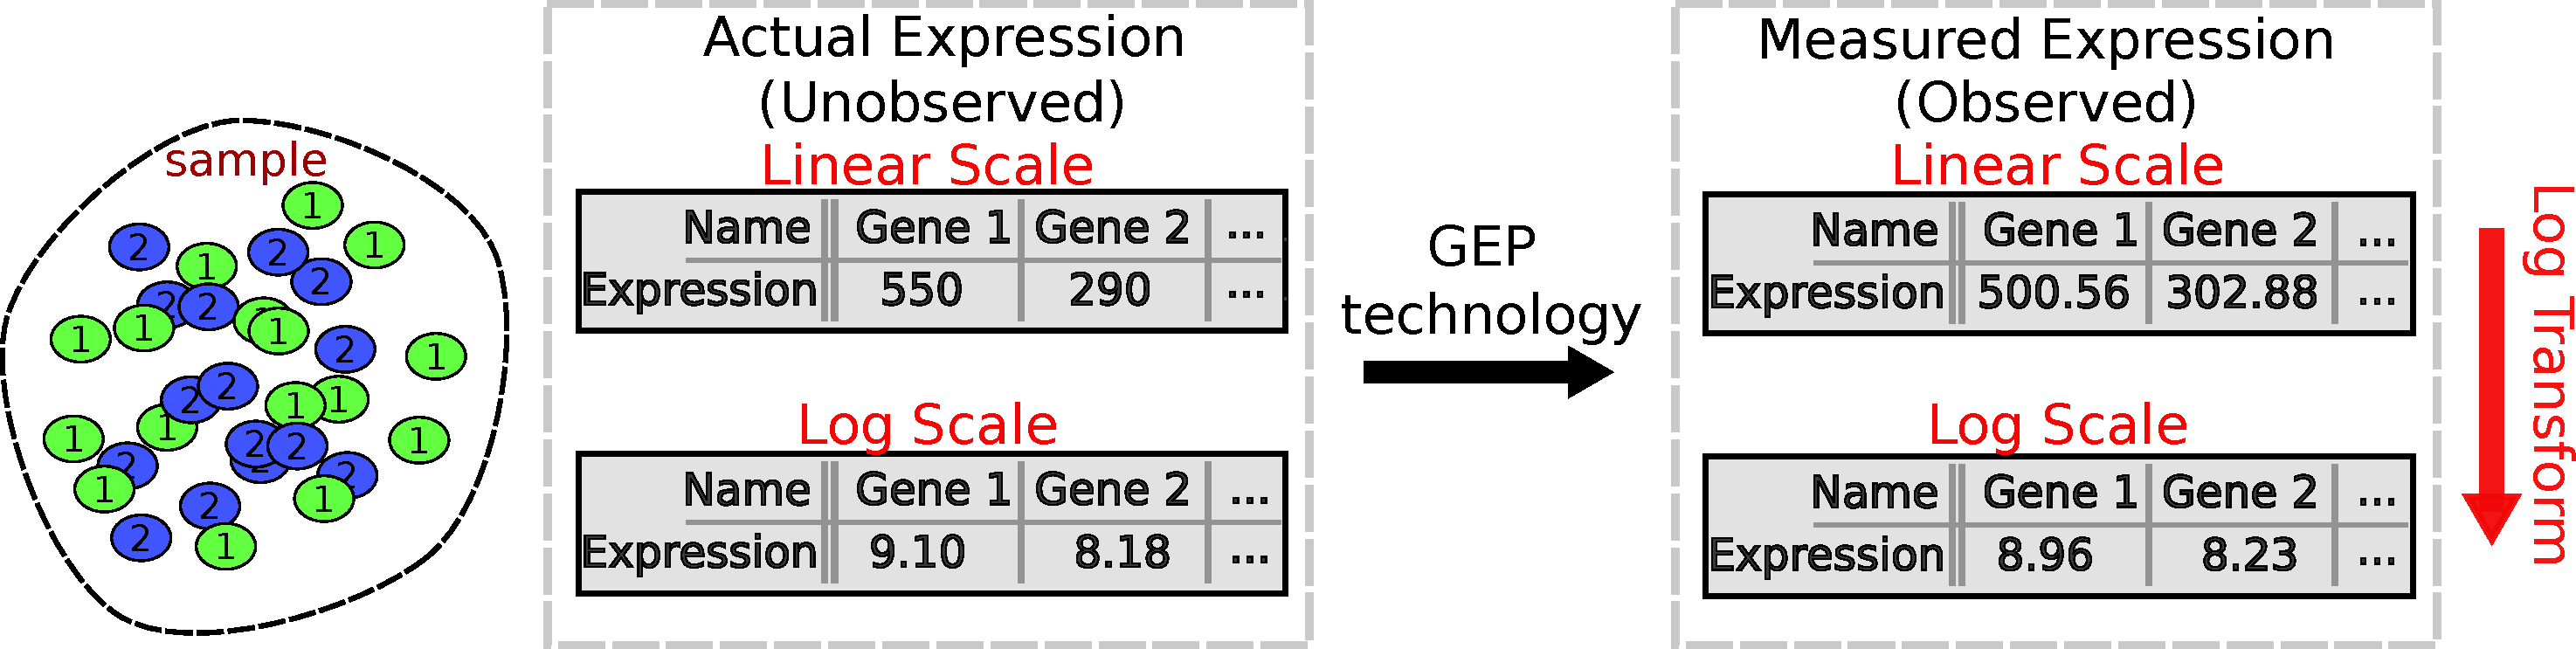
\includegraphics[scale=.24]{pictures/termscales}
  \end{figure}
  \end{center}

  \hspace*{-1cm}\vspace{-1cm}\begin{enumerate}
  \uncover<2->{\item {\bf Existing approach:} model and fit measured exprs. as $M=PR+E$ on \alert{linear} or \alert{$\log$} scale}
  \uncover<3->{\hspace*{-1.75cm}\item {\bf dtangle's approach:}}
  \begin{enumerate}
    \uncover<3->{\item[(1)] model actual exprs. as $M=PR$ on \alert{linear} scale \uncover<4->{{\bf\color{blue} (biologically plausible)}}}
    \uncover<5->{\item[(2)] model GEP tech. as linear on \alert{$\log$-$\log$} scale \uncover<6->{{\bf\color{blue} (statistically efficient)}} }
    \uncover<7->{\item[(3)] combine and simplify (1) and (2) with \alert{marker genes}, fit on \alert{$\log$} scale \uncover<8->{{\bf\color{blue} (plausible, robust, closed form, fast)}}}
  \end{enumerate}
  \end{enumerate}
\end{frame}

\begin{frame}
  \frametitle{dtangle's approach}  
  {\bf\large (Step 1)} model mixing of \alert{actual} expressions on the \alert{linear} scale:
  \[\ecna = \text{actual expression  of gene {\cbr \na} in {\crb mixture sample}}\](and similarly for $\eana$ and $\ebna$ etc.),
  \[
  \ecna=\pa\eana+\pb\ebna.
  \]
  \uncover<2->{{\bf\large (Step 2)} model GEP tech. as linear on \alert{$\log$-$\log$} scale:\\
    \begin{overprint}
      \onslide<2-3>\[\begin{aligned}\ycna &= \tna + \slope\log_2\left(\ecna\right)+\epscna\\\yana &= \tna + \slope\log_2\left(\eana\right)+\epsana\\\end{aligned}\]
      \onslide<4>\[\begin{aligned}\ycna &= \tna + \slope\log_2\left(\pa\eana+\pb\ebna\right)+\epscna\\\yana &= \tna + \slope\log_2\left(\eana\right)+\epsana\\\end{aligned}\]
      \onslide<5>\[\begin{aligned}\ycna &= \tna + \slope\log_2\left(\pa\eana\right)+\epscna\\\yana &= \tna + \slope\log_2\left(\eana\right)+\epsana\\\end{aligned}\]
      \onslide<6>\[\frac{\ycna-\yana}{\slope} = \log_2\left(\pa\right)+\epsilon\]
      \onslide<7->\[\exp_2\left(\frac{\ycna-\yana}{\slope}\right) \approx \pa\]
    \end{overprint}
  }
  \uncover<3->{{\bf\large (Step 3)} define marker genes: $\eanb=0\text{ and }\ebna=0$}
\end{frame}

\begin{frame}
Instead of estimating $\pa$ with $\exp_2\left(\frac{\ycna-\yana}{\slope}\right)$ and $\pb$ with $\exp_2\left(\frac{\ycnb-\ybnb}{\slope}\right)$
\end{frame}

\begin{frame}
  \frametitle{dtangle Models Actual Expression Mixing}
  {\bf\large Existing approach:} model mixing of \alert{measured} expressions:
  \[
  \ycn=\pa\yan+\pb\ybn
  \]
  on either the $\log$ or linear scale.
  
  \uncover<2->{{\bf\large dtangle:} model mixing of \alert{actual} expressions on the \alert{linear} scale:
  \begin{center}
    $\ecn = \text{actual expression  of gene {\cbr \n} in {\crb mixture sample}}$
    \end{center}
  (and similarly for $\ean$ and $\ebn$),
  \[
  \ecn=\pa\ean+\pb\ebn.
  \]}

  \vspace{-1cm}
  \uncover<3->{
    \alert{Compare:} $\ycn=\log_2\left(\text{measured expression  of gene {\cbr \n} in {\crb mixture sample}}\right)$
  }
\end{frame}

\begin{frame}
  \frametitle{dtangle's Models GEP Technology on the $\log$-$\log$ Scale}
  We model \alert{measured expression} on \alert{actual expression} as linear:
      \begin{overprint}
      \onslide<1|handout:0>\begin{overpic}[scale=.23,tics=10]{pictures/ma_mod_plot_empty} \put (-6,50) {} \put (11,10) {} \end{overpic}
      \onslide<2-|handout:0>\begin{overpic}[scale=.23,tics=10]{pictures/ma_mod_plot} \put (-10,45) {\alert{$M_{\n}$}} \put (50,-5) {$\log_2$\alert{$\widetilde{M}_{\n}$}} \end{overpic}
      \end{overprint}
\uncover<3->{\hspace*{3.5cm}\begin{minipage}{\textwidth}\vspace*{-6cm}\[
      \begin{aligned}
        \yan &= \tn + \slope\log_2\left(\ean\right)+\epsan\\
        \ybn &= \tn + \slope\log_2\left(\ebn\right)+\epsbn\\
        \ycn &= \tn + \slope\log_2\left(\ecn\right)+\epscn
      \end{aligned}
      \]
      \end{minipage}}
\end{frame}

\begin{frame}
  \frametitle{dtangle's Rigorously Defines Marker Genes}
  
  \alert{(Defn) Marker gene:} acutally expressed in only one type.\\
  i.e. $\eanb=0\text{ and }\ebna=0$.

 \uncover<2->{{\bf Combining this definition with our models:}}
  
  \uncover<2->{\fbox{\alert{Mixing Model:} $\ecn=\pa\ean+\pb\ebn$}}
  \begin{overprint}
    \onslide<3|handout:0>\[\ycn = \tn + \slope\log_2\left(\ecn\right)+\epscn\]
    \onslide<4-|handout:0>\[\ycn = \tn + \slope\log_2\underbrace{\left(\pa\ean+\pb\ebn\right)}_{\ecn}+\epscn\]
  \end{overprint}

  \uncover<5->{\fbox{\alert{Marker Gene Defn:} $\eanb=0\text{ and }\ebna=0$}}\vspace{-.25cm}
  \begin{overprint}
    \onslide<6|handout:0>\[\ycna = \tna + \slope\log_2\left(\pa\eana+\pb\eanb \right)+\epsilon_{\cbr a}\]
    \onslide<7|handout:0>\[\ycna = \tna + \slope\log_2\left(\pa\eana+\hcancel[red]{\color{gray}\pb\eanb} \right)+\epsilon_{\cbr a}\]
    \onslide<8|handout:0>\[\ycna = \tna + \slope\log_2\left(\pa\eana\right)+\epsilon_{\cbr a}\]
  \end{overprint}
  \begin{overprint}
    \onslide<6|handout:0>\[\ycnb = \tnb + \slope\log_2\left(\pa \ebna+\pb\ebnb\right)+\epsilon_{\cbr b}\]
    \onslide<7|handout:0>\[\ycnb = \tnb + \slope\log_2\left(\hcancel[red]{{\color{gray} \pa\ebna}}+\pb\ebnb\right)+\epsilon_{\cbr b}\]
    \onslide<8|handout:0>\[\ycnb = \tnb + \slope\log_2\left(\pb\ebnb\right)+\epsilon_{\cbr b}\]
  \end{overprint}

\end{frame}

\begin{frame}
    \frametitle{dtangle's Makes Two Simple Assumptions}
    Using these we have that
    
    $\ycna-\ycnb$\vspace{.1cm}
    \begin{overprint}
      \onslide<1|handout:0>\vspace{.1cm}$=\slope\log_2\left(\nicefrac{\pa}{\pb}\right)+\text{{\Huge $\ldots$}}$
      \onslide<2-|handout:0>$=\slope\log_2\left(\nicefrac{\pa}{\pb}\right)+\underbrace{\slope\log_2\left(\nicefrac{\eana}{\ebnb}\right) +\left(\tna-\tnb\right)}_{\alert{\text{Need to Adjust For These Terms}}} +\left(\epsilon_{\cbr a} -\epsilon_{\cbr b}\right)$
      \end{overprint}
    
    \uncover<3->{
      
      however
      
$\yana - \ybnb$
$=\underbrace{\slope\log_2\left(\nicefrac{\eana}{\ebnb}\right)+\left(\tna -\tnb\right)}+\left(\epsilon_{\crb A \cbr a}  +\epsilon_{\crb B \cbr b}\right)$}

    \uncover<4->{\alert{Solution:} adjust $\ycna-\ycnb$ with $\yana - \ybnb$ to get\vspace{-.25cm}
{\Large \[\boxed{
\left(\ycna-\ycnb\right)-\left(\yana - \ybnb\right) = \slope\log_2\left(\nicefrac{\pa}{\pb}\right)+\epsilon
  }\]}
    }

    \begin{center}\vspace{-1cm}
      \uncover<5->{\alert{Next:} solve for $\pa$ and $\pb$}
      \end{center}

\end{frame}

\begin{frame}
  \frametitle{The {\bf dtangled} Estimators Can Be Derived from Our Model}
  Thus it can be shown that
  \[
  \logistic_2\left(\frac{\left(\yca-\ycb\right)-\left(\yaa-\ybb\right)}{\slope}\right) \approx \pa
  \]
  and similarly for $\crb B$.

  \alert{The {\bf dtangled} estimators come naturally from our model:}\\
  \hspace{.5cm}$\widehat{\pa}$ and $\widehat{\pb}$ are the plug-in estimators replacing $\slope$ with $\slopehat$,
    \[
\widehat{\pa} = \logistic_2\left(\frac{\left(\yca-\ycb\right)-\left(\yaa-\ybb\right)}{\slopehat}\right)\approx \pa
\]
\fbox{This can all be generalized to multiple cell types, references, markers.}
\end{frame}

\begin{frame}
  \frametitle{Loose Ends: Marker Genes and $\gamma$}
  \begin{enumerate}
  \item Estimate $\slope$ from \alert{benchmark data sets}:
    \hspace*{2cm}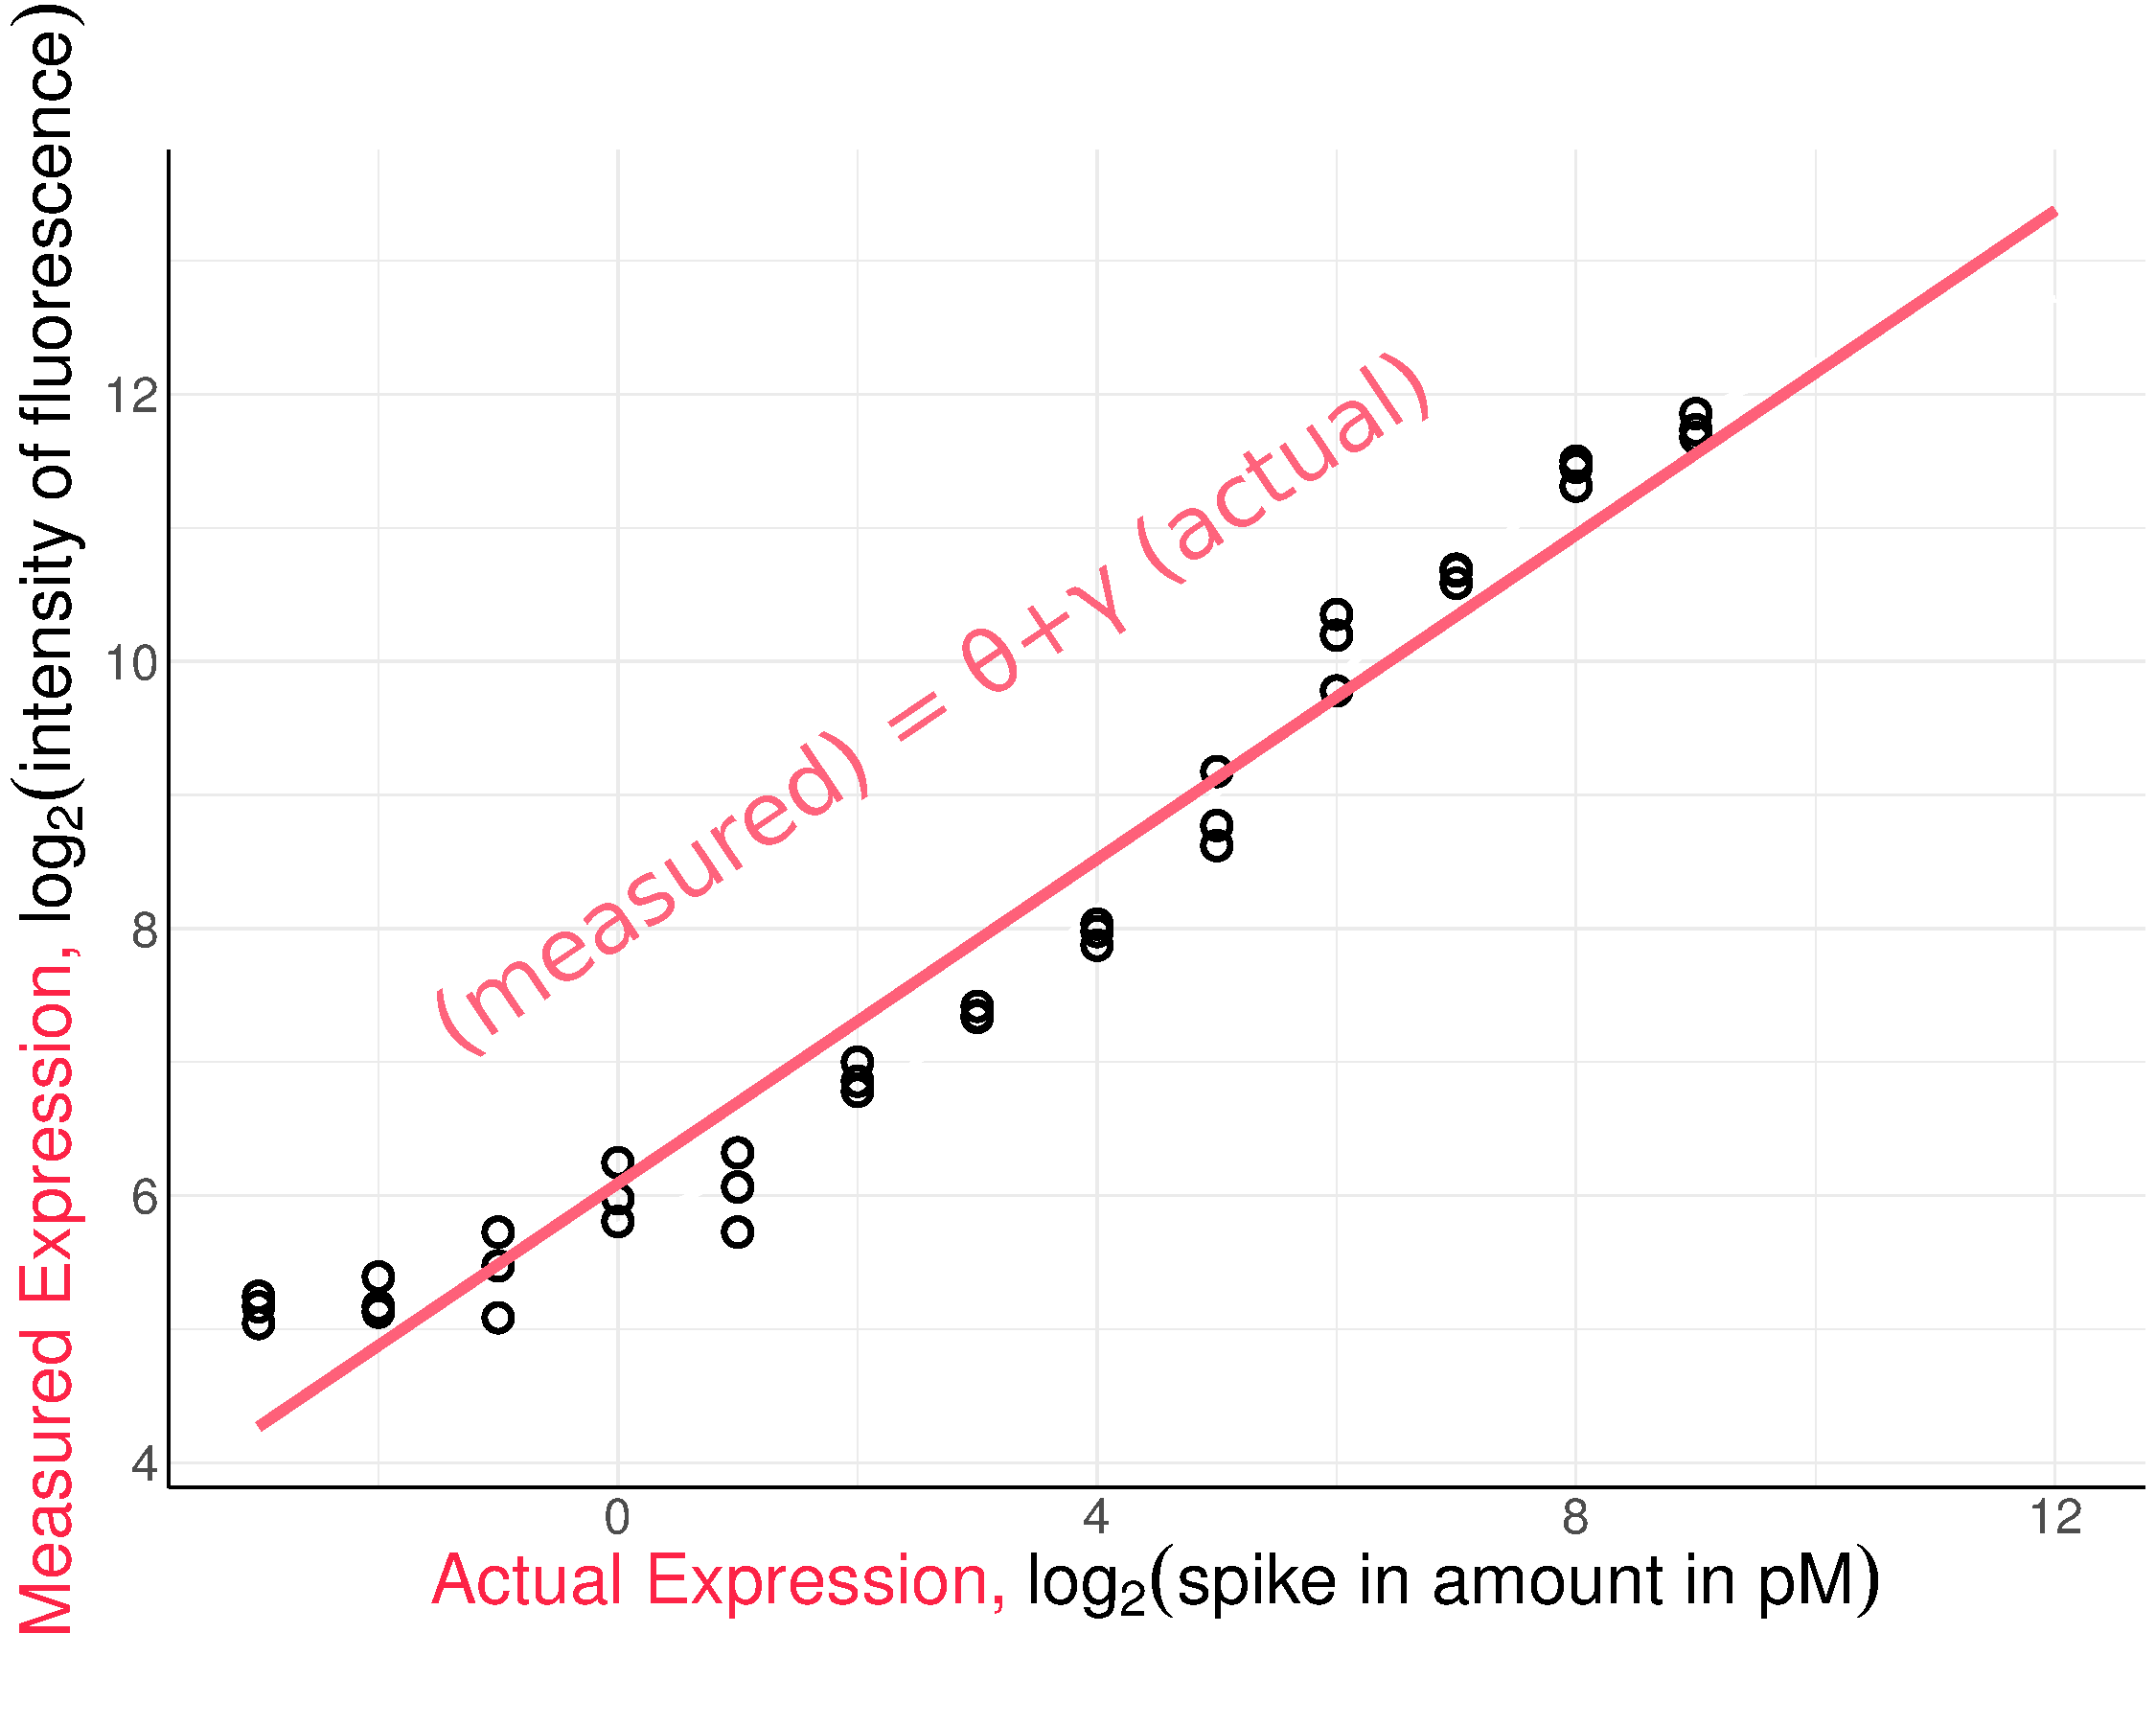
\includegraphics[scale=.17]{pictures/ma_mod_plot}
  \item We find \alert{marker genes} through \alert{differential expression analysis} on the references.
  \end{enumerate}
  {\bf dtangle robust to changes in $\gamma$ and marker genes.}
\end{frame}

%\begin{frame}
%  \frametitle{Contrast with the Literature}
%  There are two major points at which {\bf dtangle} departs from the literature.
%  
%  \begin{enumerate}
%  \item \alert{The Model and Unknown Parameters}\\{\bf dtangle}: unknown $p_{\crb k},\eta_{\crb k\cbr n},\tn$ and $\gamma$
%    \[
%Y_{\cbr n} = \theta_{\cbr n} + \gamma \log_2\left(\sum_{{\crb k}=1}^{{\crb K}}p_{\crb k}\eta_{\crb k \cbr n}\right),\quad Z_{{\crb k}r \cbr n} = \theta_{\cbr n} + \gamma \log_2\left(\eta_{\crb k \cbr n}%\right)
%\]
%effective model in the literature: unknown $p_{\crb k}$\\
%\vspace{-.4cm}\[
%\exp_2(Y_{\cbr n}) = \sum_{{\crb k}=1}^{{\crb K}}p_{\crb k}\exp_2\left(Z_{{\crb k}r \cbr n}\right) \text{ or } Y_{\cbr n} = \sum_{{\crb k}=1}^{{\crb K}}p_{\crb k}Z_{{\crb k}r \cbr n}
%\]
%\item \alert{Fitting The Algorithm} \\{\bf dtangle}: (1) make assumptions about markers (2) estimate $\gamma$ separately (3) normalize  and solve directly for $p_{\crb k}$\newline
%  {\bf literature}: (1) regression or (2) bayesian
%  \end{enumerate}
%\end{frame}

\setcounter{subsection}{0}
\section{Analysis}
\subsection{}

\begin{frame}
  \frametitle{dtangle Works Well (Shen-Orr et al.)}
  \begin{figure}
   \hspace*{-1cm}
  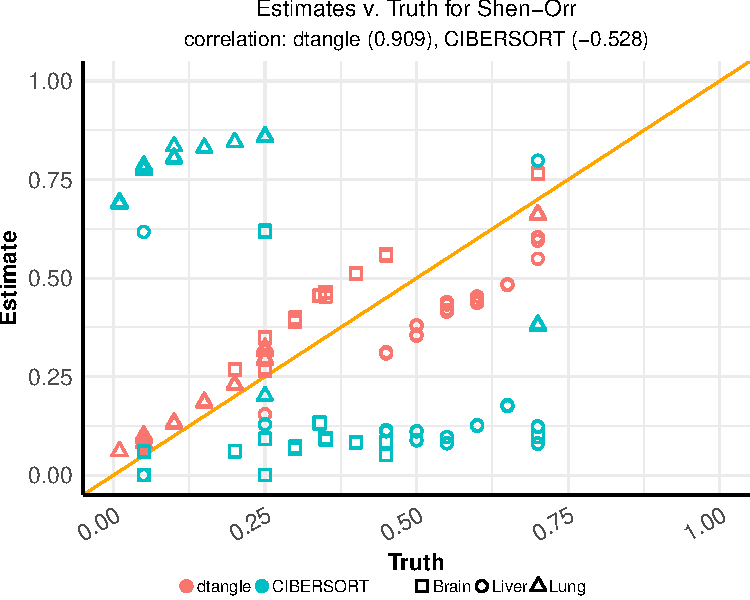
\includegraphics[scale=.75]{pictures/Shen-Orr_scatter.pdf}
  \end{figure}
\end{frame}


\begin{frame}
  \frametitle{dtangle Works With Complicated Data (Becht et al.)}
  \begin{figure}
   \hspace*{-1cm}
  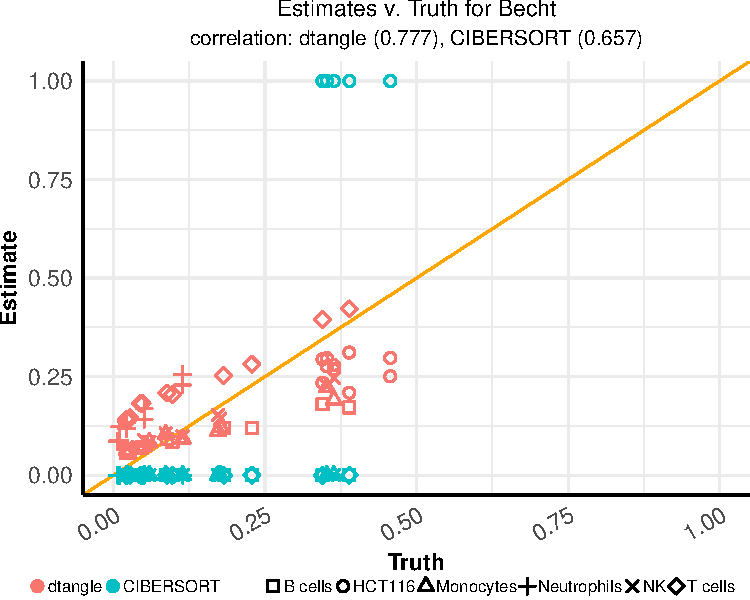
\includegraphics[scale=.75]{pictures/Becht_scatter.pdf}
  \end{figure}
\end{frame}

\begin{frame}
  \frametitle{dtangle is Consistently Good}
  \begin{figure}
  \hspace*{-1cm}
  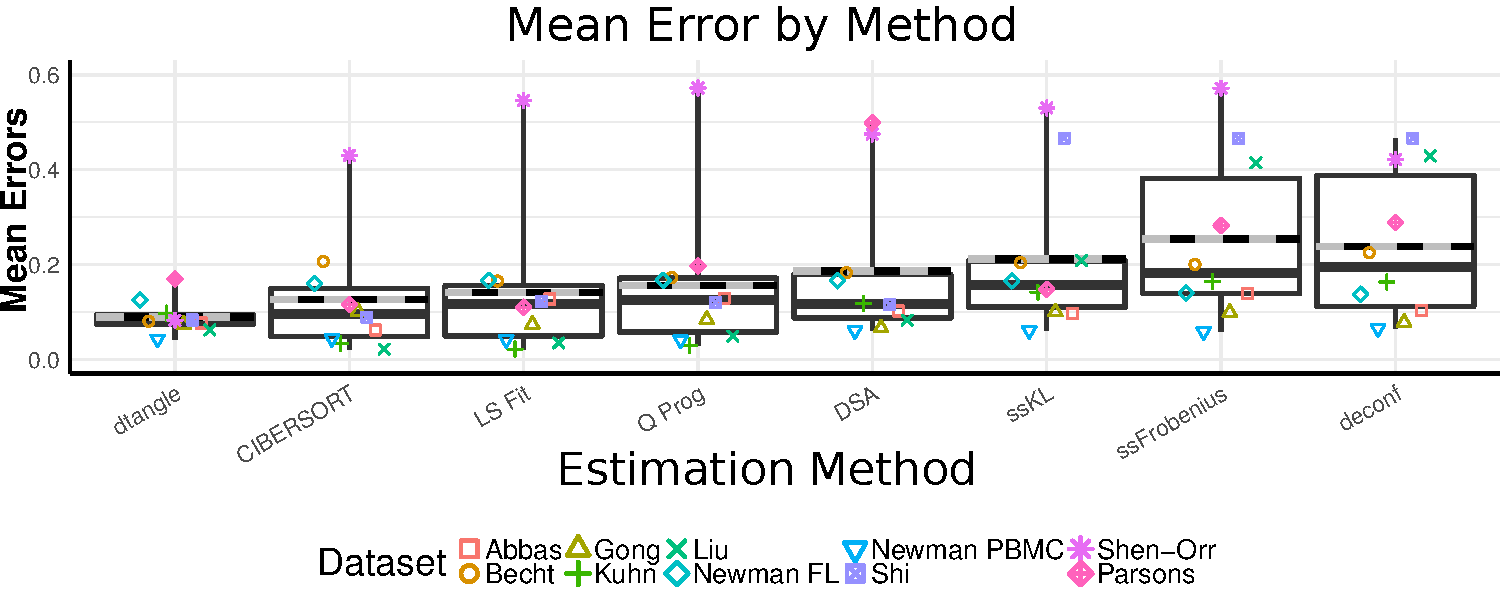
\includegraphics[scale=.499]{pictures/meta_boxplots.pdf}
  \end{figure}
\end{frame}

\begin{frame}
  \frametitle{dtangle is Fast}
  \begin{figure}
  \hspace*{-1cm}
  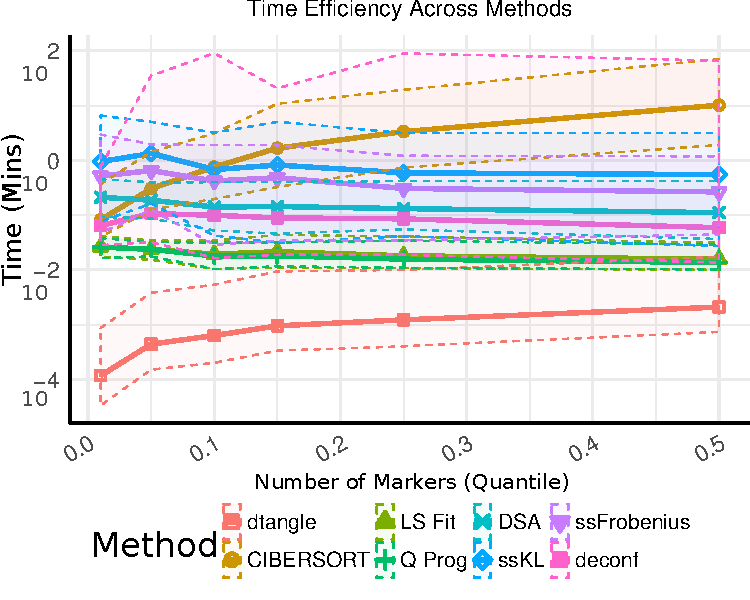
\includegraphics[scale=.8]{pictures/time_plot.pdf}
  \end{figure}
\end{frame}

\begin{frame}
  \frametitle{Revisiting the Lyme Example}
  {\bf Gene expression measurements (RNA-seq) of PBMCs from Bouquet et al.}

  \begin{enumerate}
  \item Gene expression measurements of PBMCs (subset of white-blood cells) of 28 patients at three points:
  \begin{enumerate}
  \item[\cbo(V1)] the point of acute Lyme disease diagnosis
  \item[\cbo(V2)] immediately after the completion of a 3-week course of doxycycline
  \item[\cbo(V5)] 6 months after completion of the doxycycline
  \end{enumerate}
  \item Gene expressions of PBMCs from 13 matched (healthy) controls were also collected {\cbo(C)}
  \end{enumerate}

\end{frame}

\begin{frame}
  \frametitle{dtangle on the Lyme data}
  \vspace*{-.5cm}\begin{figure}
    \hspace*{-.9cm}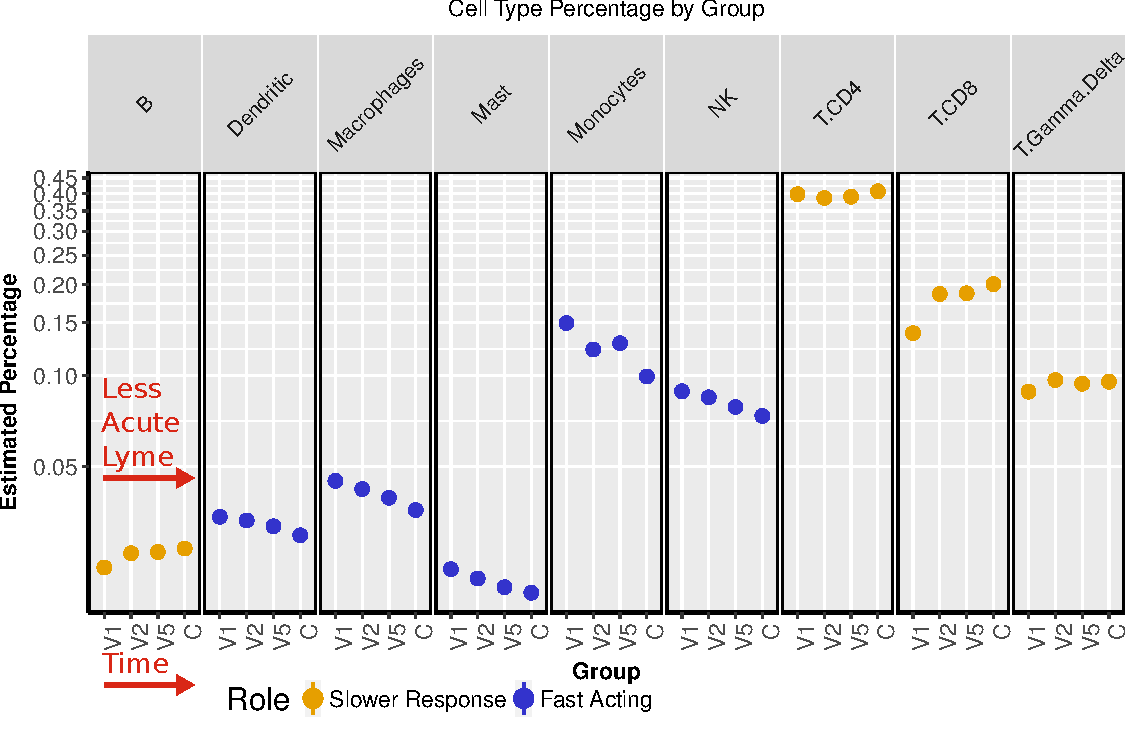
\includegraphics[scale=.65]{pictures/ctypes.pdf}
  \end{figure}
\end{frame}

\begin{frame}
  \frametitle{dtangle on the Lyme data}
  \vspace*{-.9cm}\begin{figure}
    \hspace*{-.9cm}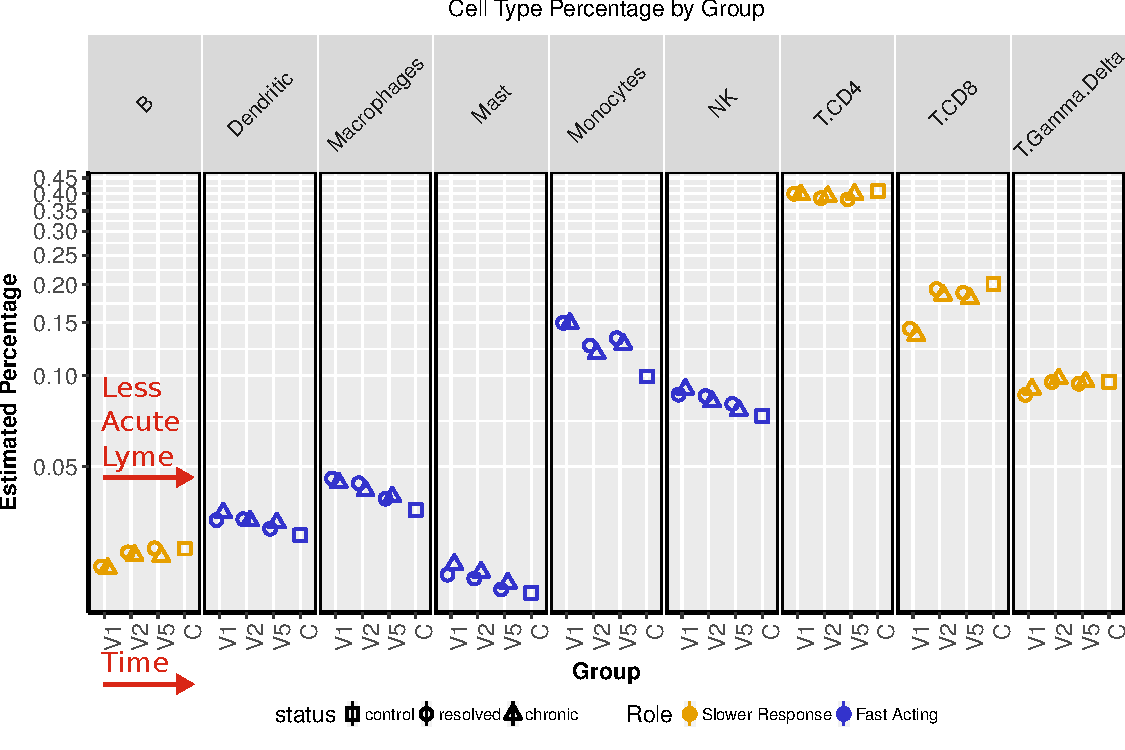
\includegraphics[scale=.37]{pictures/ctypes2.pdf}
  \end{figure}
\end{frame}

\begin{frame}
  \frametitle{Accounting for Cell Types Drastically Changes Results}
  Following Bouquet et al. (2016) we compare the control group to V1, V2 and V5.

  We find that
  \begin{enumerate}
    \item {\bf unadjusted:} there are {\cbo 399} genes that are differentially expressed in the intersection of each of the three comparisons
    \item {\bf cell-type adjusted:} adding in covariates to account for the fast-acting cell types (phagocyte and NK) reduces the differentially expressed genes to only {\cbo 158}
  \end{enumerate}
\end{frame}

\backupbegin

\begin{frame}
  \frametitle{dtangle is available!}
{\Large
  \begin{center}
    On github\\
    \alert{\url{dtangle.github.io}}\\
    or on CRAN\\
    \alert{\url{cran.r-project.org/package=dtangle}}\\\vspace{1cm}
      Hopefully rolling out to stemformatics soon!\\
      \alert{\url{www.stemformatics.org}}

      \uncover<2->{\fbox{\color{blue} Thanks!}}
  \end{center}
}
\end{frame}

\begin{frame}
  \frametitle{We Have Many Ideas for Improving dtangle!}
  {\bf There are several ways we are looking at extending dtangle:}
  \begin{enumerate}
  \item variance and goodness-of-fit 
  \item estimating proportion of unknown cell-types
  \item removing unwanted latent factors as part of deconvolution
  \item extension to high-throughput methylation data
  \end{enumerate}
\end{frame}

\begin{frame}
  \frametitle{dtangle is Generaliziable}
The general deconvolution setting is
  \begin{enumerate}
  \item $\cK$ cell types
  \item $\nu_{\crb k}$ pure samples of type $\crb k$
  \item $\log$-level expression data for each pure sample
  \[
Z_{{\crb k}r} \in \mathbb{R}^{1\times \cbr N},\quad r=1,\ldots,\nu_{\crb k}.
\]
\item Set of marker genes $\cbr G_{k}$ for each cell type
  \item Mixture sample of $\cK$ cell types in proportions $p_{\crb 1},\ldots,p_{\crb K}$
\item $\log$-level expression measurements of mixture sample: $Y_{\cbr n}$
\end{enumerate}
\end{frame}

\begin{frame}
  \frametitle{General Estimators Look Similar}
  For the simple case we had
  \[
\widehat{p_{\crb A}} = \logistic_2\left(\frac{\left(\yca-\ycb\right)-\left(\yaa-\ybb\right)}{\slopehat}\right)
\]
in the general case we have a direct generalization
\vspace{-.35cm}\[\hspace{-.75cm}\boxed{
  \widehat{p_{\crb k}} = L_{\crb k}\left(\frac{\left(\ykbar - \overline{Y_{\cbr G_1}}\right) - \left(\zkbar-\overline{Z_{\cbr G_1}}\right)}{\slopehat},\ldots,\frac{\left(\ykbar - \overline{Y_{\cbr G_K}}\right) - \left(\zkbar-\overline{Z_{\cbr G_K}}\right)}{\slopehat}\right)}
\]
  \vspace{-.25cm}with
  \begin{enumerate}
  \item $\ykbar = \frac{1}{|{\cbr G_{k}}|}\sum_{\cbr n\in G_k}Y_{\cbr n}$, average marker genes in the mixture sample
  \item $\zkbar = \frac{1}{|{\cbr G_{k}}|\nu_{\crb k}}\sum_{\cbr n\in G_k}\sum_{r=1}^{\nu_{\crb k}}Z_{{\crb k}r{\cbr n}}$, average marker genes in pure samples 
  \item $L_{\crb k}(x) = \nicefrac{1}{\left(1+\sum_{t\neq {\crb k}} 2^{-x_t}\right)}$, a generalized logistic function
  \end{enumerate}
\end{frame}

\begin{frame}
  \frametitle{Image Attribution}
  \begin{enumerate}
  \item [1] Adult deer tick, ``Ixodes scapularis''.;Source: \url{http://www.ars.usda.gov/is/graphics/photos/mar98/k8002-3.htm};Image Number: K8002-3 ;Credits: Photo by Scott Bauer. PD-USGov-USDA-ARS
  \item [2] Electron micrograph of ``Treponema pallidum''. From \url{http://phil.cdc.gov/phil/home.asp} ID 1977. 
  \end{enumerate}
\end{frame}

\begin{frame}[allowframebreaks]
\bibliography{/home/greg/Dropbox/work/research/bibtex/Deconvolution,/home/greg/Dropbox/work/research/bibtex/Other}
\end{frame}

\backupend

\end{document}
